\subsubsection{Schaltungsaufbau} \label{subsec:schaltungsaufbau}

Das vorgegebene EMI-Filter muss bezüglich der Einfügungsverluste (Insertion Loss) untersucht werden. Die Einfügunsverluste hängen vom Gesamtrauschen der Schaltung ab. Es wird ein Ansatz verwendet, der in der Praxis weit verbreitet ist, bei welchem das Gesamtrauschen in zwei Komponenten unterteilt wird. Man spricht vom Gegen-(=Differential Mode=DM) und Gleichtaktrauschen (=Common Mode=CM). Anhand der vorgegebenen CM- und DM-Äquivalenten Schaltungen (Abbildungen \ref{fig:CM-Schaltungäquivalent}, \ref{fig:DM-Schaltungsäquivalent})werden die Einfügungsverluste in Funktion der Frequenz berechnet. Die Berechnungen decken einen Bereich von 0 bis 30MHz ab. 


 
\newpage

Die Schaltung \ref{fig:orig_Schaltung} \nameref{fig:orig_Schaltung} zeigt den Filteraufbau, wie er der Aufgabenstellung zu entnehmen ist. Um das Gegentaktrauschen und das Gleichtaktrauschen bestimmen zu können, werden die beiden Schaltungsäquivalente gebildet. 
\begin{figure}[H]
	\centering
	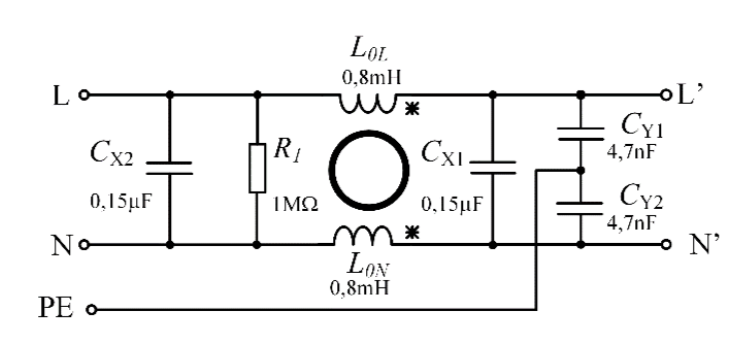
\includegraphics[width = 10cm]{orig_ElectricalCircuit.png}
	\caption{Original Schaltung \cite{aufgabenstellung}}
	\label{fig:orig_Schaltung}
\end{figure}
Hierbei müssen die elektrischen Bauelemente, wie Spule und Kondensator mit den passenden parasitären Parameter ergänz werden. In Abbildung \ref{fig:stray_L} und \ref{fig:stray_C} werden die parasitären Parameter von Spule und Kondensator gezeigt.
\begin{figure}[H]
	\begin{minipage}[h]{0.45\linewidth}
		\centering
		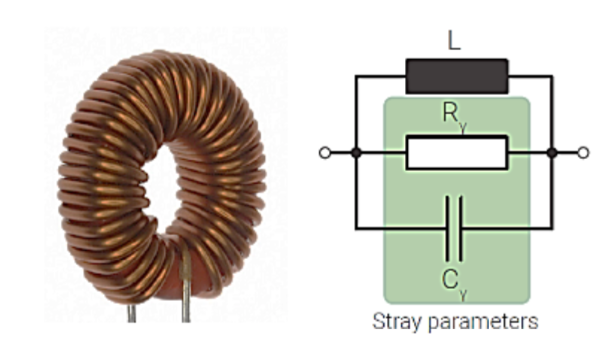
\includegraphics[width = 5cm]{stray_L.png}
		\label{fig:stray_L}
		\caption{Parasiäre Elemente einer Induktivität \cite{aufgabenstellung}}
	\end{minipage}
	\begin{minipage}[h]{0.45\linewidth}
		\centering
		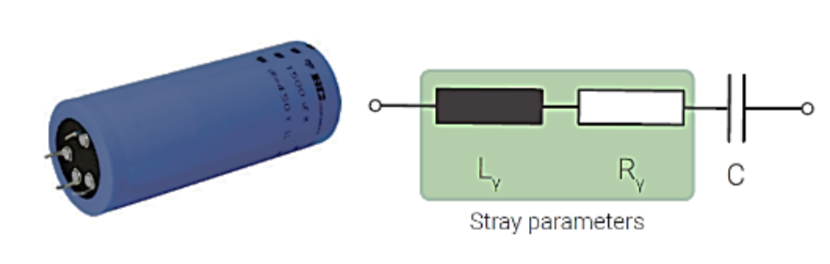
\includegraphics[width = 7cm]{stray_C.png}
		\label{fig:stray_C}
		\caption{Parasiäre Elemente einer Kapazität \cite{aufgabenstellung}}
	\end{minipage}
\end{figure}
Folgende Schaltungen stellen die CM- und DM-Äquivalenten Schaltungen. Da die Berechnungen in einem Bereich von bis zu 30 MHz gemacht werden, ist es notwendig die parasitären Parameter von Spule und Kondensator miteinzubeziehen.

\begin{figure}[H]
	\centering
	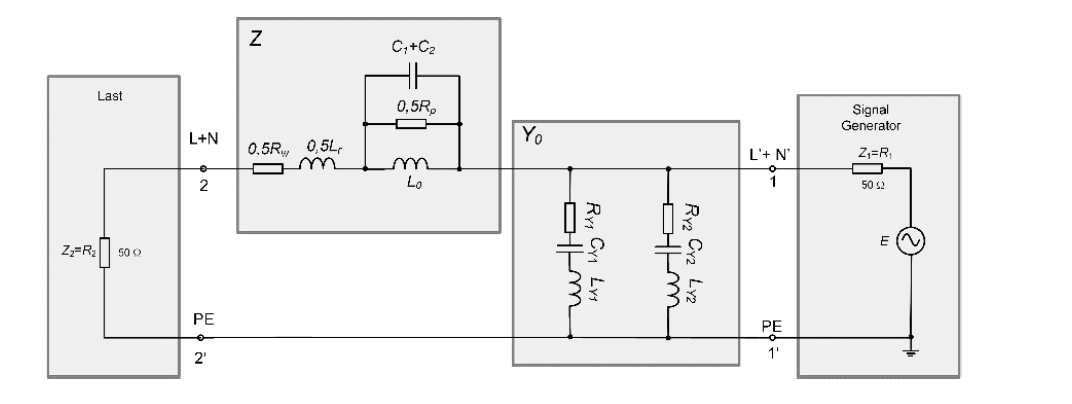
\includegraphics[width=15cm]{CM_ElectricalCircuit.png}
	\caption{CM-Schaltungäquvalent \cite{aufgabenstellung}}
	\label{fig:CM-Schaltungäquivalent}
\end{figure}

\begin{figure}[H]
	\centering
	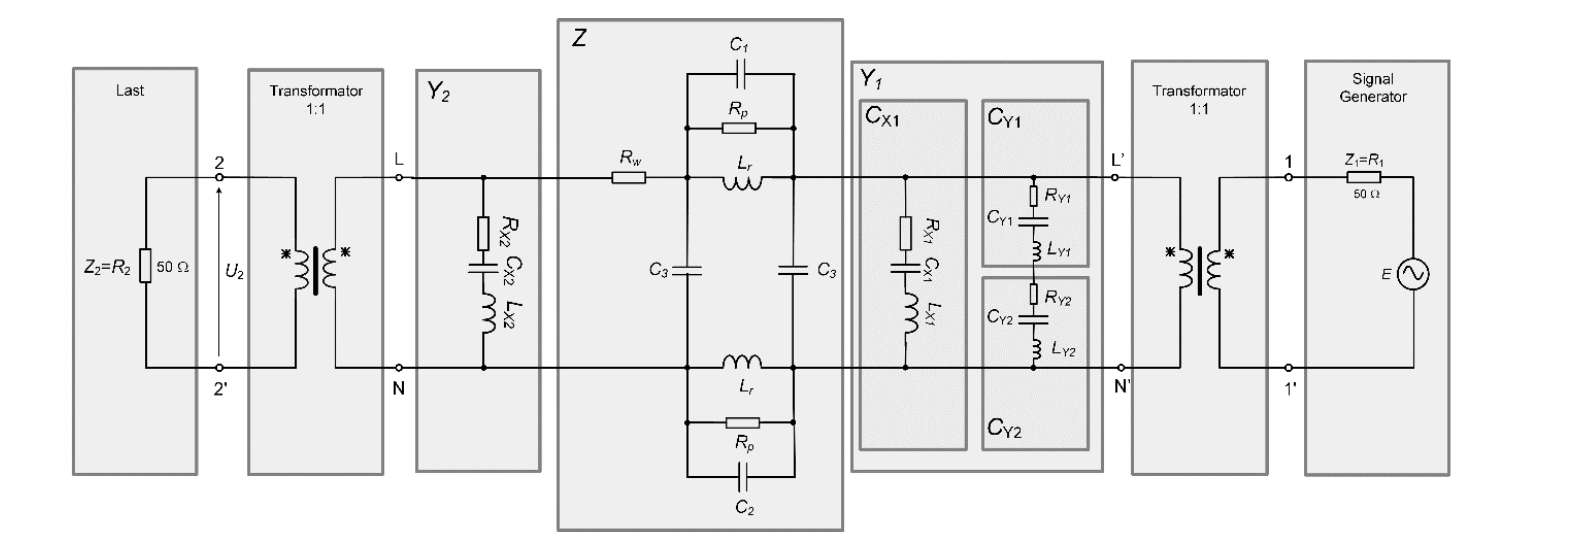
\includegraphics[width=15cm]{DM_ElectricalCircuit.png}
	\caption{DM-Schaltungsäquvalent \cite{aufgabenstellung}}
	\label{fig:DM-Schaltungsäquivalent}
\end{figure}
\newpage

%TODO Die Schaltungsäquivalenzen müssen aufgeteilt werden und in die jeweiligen subsubsections gekippt werden
